\problemname{Tivoli}

Lisa er kommet til tivoli og har bestemt sig for at prøve $N$ attraktioner en gang hver.
Hver attraktion er anlagt to gange, og de to anlæg er lige gode; totalt findes der altså $2N$ anlæg.
Givet positionerne for samtlige anlæg, hjælp Lisa med at planlægge, hvilke $N$ anlæg hun skal vælge og i hvilken rækkefølge for at minimere den strækning, hun skal gå for at besøge alle $N$ attraktioner.

Desuden begynder og slutter hun ved indgangen.
Indgangen er i origo, $(0,0)$.

I eksemplet forneden er $N=3$, og de to anlæg af attraktion $a$ kaldes $a_1$ og $a_2$.
Lisa går fra indgangen til $2_2$, derfra til $1_1$, så til $3_1$ og endelig tilbage til indgangen.
Den totale strækning er $14{,}23345$.

\bigskip
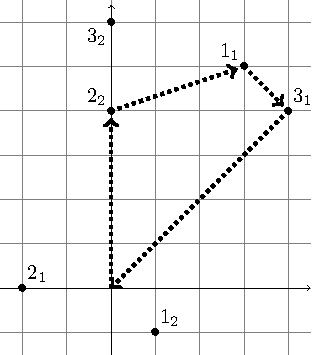
\includegraphics{img/tivoli-sample-img.pdf}

\section*{Indlæsning}
Første linje består af heltallet $N$, antallet af attraktioner, som Lisa vil besøge ($1 \le N \le 15$).
Derefter følger $N$ linjer, hvoraf første linje beskriver attraktion nummer~$1$, anden linje beskriver attraktion nummer $2$, osv.
Hver linje indeholder fire heltal: $x$- og $y$-koordinaterne for denne attraktions første anlæg efterfulgt af $x$- og $y$-koordinaterne for denne attraktions andet anlæg.
Koordinaternes absolutværdi er mindre end en million.

Intet anlæg er på samme plads som noget andet.
Intet anlæg er i origo.

\section*{Udskrift}
Udlæsningens første linje skal bestå af et decimaltal skrevet med decimalpunktum: hvor langt Lisa skal gå. 
Derefter skal komme $N$ linjer med to heltal på hver, attraktionsnummeret (mellem $1$ og $N$) og anlægsnummeret ($1$ eller $2$).

Den første af de $N$ linjer fortæller altså, hvilket anlæg hun skal besøge først, og den sidste linje fortæller, hvilket anlæg hun skal besøge sidst.
Hvis der findes flere veje med lige kort strækning (fx ved at følge en løsning baglæns), kan du vælge hvilken som helst af dem.
Læg mærke til, at det først udskrevne decimaltal skal tage hensyn til, at Lisa skal begynde og slutte ved indgangen.

Den relative fejl skal være mindre end $10^{-5}$.
